\documentclass[1p]{elsarticle_modified}
%\bibliographystyle{elsarticle-num}

%\usepackage[colorlinks]{hyperref}
%\usepackage{abbrmath_seonhwa} %\Abb, \Ascr, \Acal ,\Abf, \Afrak
\usepackage{amsfonts}
\usepackage{amssymb}
\usepackage{amsmath}
\usepackage{amsthm}
\usepackage{scalefnt}
\usepackage{amsbsy}
\usepackage{kotex}
\usepackage{caption}
\usepackage{subfig}
\usepackage{color}
\usepackage{graphicx}
\usepackage{xcolor} %% white, black, red, green, blue, cyan, magenta, yellow
\usepackage{float}
\usepackage{setspace}
\usepackage{hyperref}

\usepackage{tikz}
\usetikzlibrary{arrows}

\usepackage{multirow}
\usepackage{array} % fixed length table
\usepackage{hhline}

%%%%%%%%%%%%%%%%%%%%%
\makeatletter
\renewcommand*\env@matrix[1][\arraystretch]{%
	\edef\arraystretch{#1}%
	\hskip -\arraycolsep
	\let\@ifnextchar\new@ifnextchar
	\array{*\c@MaxMatrixCols c}}
\makeatother %https://tex.stackexchange.com/questions/14071/how-can-i-increase-the-line-spacing-in-a-matrix
%%%%%%%%%%%%%%%

\usepackage[normalem]{ulem}

\newcommand{\msout}[1]{\ifmmode\text{\sout{\ensuremath{#1}}}\else\sout{#1}\fi}
%SOURCE: \msout is \stkout macro in https://tex.stackexchange.com/questions/20609/strikeout-in-math-mode

\newcommand{\cancel}[1]{
	\ifmmode
	{\color{red}\msout{#1}}
	\else
	{\color{red}\sout{#1}}
	\fi
}

\newcommand{\add}[1]{
	{\color{blue}\uwave{#1}}
}

\newcommand{\replace}[2]{
	\ifmmode
	{\color{red}\msout{#1}}{\color{blue}\uwave{#2}}
	\else
	{\color{red}\sout{#1}}{\color{blue}\uwave{#2}}
	\fi
}

\newcommand{\Sol}{\mathcal{S}} %segment
\newcommand{\D}{D} %diagram
\newcommand{\A}{\mathcal{A}} %arc


%%%%%%%%%%%%%%%%%%%%%%%%%%%%%5 test

\def\sl{\operatorname{\textup{SL}}(2,\Cbb)}
\def\psl{\operatorname{\textup{PSL}}(2,\Cbb)}
\def\quan{\mkern 1mu \triangleright \mkern 1mu}

\theoremstyle{definition}
\newtheorem{thm}{Theorem}[section]
\newtheorem{prop}[thm]{Proposition}
\newtheorem{lem}[thm]{Lemma}
\newtheorem{ques}[thm]{Question}
\newtheorem{cor}[thm]{Corollary}
\newtheorem{defn}[thm]{Definition}
\newtheorem{exam}[thm]{Example}
\newtheorem{rmk}[thm]{Remark}
\newtheorem{alg}[thm]{Algorithm}

\newcommand{\I}{\sqrt{-1}}
\begin{document}

%\begin{frontmatter}
%
%\title{Boundary parabolic representations of knots up to 8 crossings}
%
%%% Group authors per affiliation:
%\author{Yunhi Cho} 
%\address{Department of Mathematics, University of Seoul, Seoul, Korea}
%\ead{yhcho@uos.ac.kr}
%
%
%\author{Seonhwa Kim} %\fnref{s_kim}}
%\address{Center for Geometry and Physics, Institute for Basic Science, Pohang, 37673, Korea}
%\ead{ryeona17@ibs.re.kr}
%
%\author{Hyuk Kim}
%\address{Department of Mathematical Sciences, Seoul National University, Seoul 08826, Korea}
%\ead{hyukkim@snu.ac.kr}
%
%\author{Seokbeom Yoon}
%\address{Department of Mathematical Sciences, Seoul National University, Seoul, 08826,  Korea}
%\ead{sbyoon15@snu.ac.kr}
%
%\begin{abstract}
%We find all boundary parabolic representation of knots up to 8 crossings.
%
%\end{abstract}
%\begin{keyword}
%    \MSC[2010] 57M25 
%\end{keyword}
%
%\end{frontmatter}

%\linenumbers
%\tableofcontents
%
\newcommand\colored[1]{\textcolor{white}{\rule[-0.35ex]{0.8em}{1.4ex}}\kern-0.8em\color{red} #1}%
%\newcommand\colored[1]{\textcolor{white}{ #1}\kern-2.17ex	\textcolor{white}{ #1}\kern-1.81ex	\textcolor{white}{ #1}\kern-2.15ex\color{red}#1	}

{\Large $\underline{12n_{0155}~(K12n_{0155})}$}

\setlength{\tabcolsep}{10pt}
\renewcommand{\arraystretch}{1.6}
\vspace{1cm}\begin{tabular}{m{100pt}>{\centering\arraybackslash}m{274pt}}
\multirow{5}{120pt}{
	\centering
	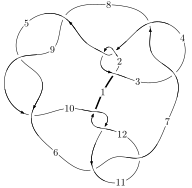
\includegraphics[width=112pt]{../../../GIT/diagram.site/Diagrams/png/2244_12n_0155.png}\\
\ \ \ A knot diagram\footnotemark}&
\allowdisplaybreaks
\textbf{Linearized knot diagam} \\
\cline{2-2}
 &
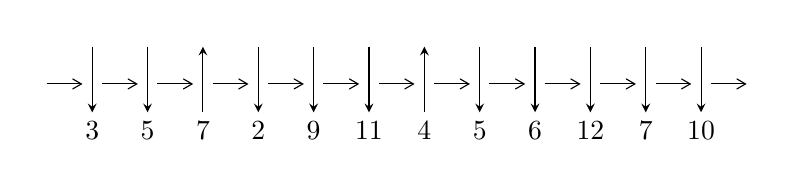
\begin{tikzpicture}[x=20pt, y=17pt]
	% nodes
	\node (C0) at (0, 0) {};
	\node (C1) at (1, 0) {};
	\node (C1U) at (1, +1) {};
	\node (C1D) at (1, -1) {3};

	\node (C2) at (2, 0) {};
	\node (C2U) at (2, +1) {};
	\node (C2D) at (2, -1) {5};

	\node (C3) at (3, 0) {};
	\node (C3U) at (3, +1) {};
	\node (C3D) at (3, -1) {7};

	\node (C4) at (4, 0) {};
	\node (C4U) at (4, +1) {};
	\node (C4D) at (4, -1) {2};

	\node (C5) at (5, 0) {};
	\node (C5U) at (5, +1) {};
	\node (C5D) at (5, -1) {9};

	\node (C6) at (6, 0) {};
	\node (C6U) at (6, +1) {};
	\node (C6D) at (6, -1) {11};

	\node (C7) at (7, 0) {};
	\node (C7U) at (7, +1) {};
	\node (C7D) at (7, -1) {4};

	\node (C8) at (8, 0) {};
	\node (C8U) at (8, +1) {};
	\node (C8D) at (8, -1) {5};

	\node (C9) at (9, 0) {};
	\node (C9U) at (9, +1) {};
	\node (C9D) at (9, -1) {6};

	\node (C10) at (10, 0) {};
	\node (C10U) at (10, +1) {};
	\node (C10D) at (10, -1) {12};

	\node (C11) at (11, 0) {};
	\node (C11U) at (11, +1) {};
	\node (C11D) at (11, -1) {7};

	\node (C12) at (12, 0) {};
	\node (C12U) at (12, +1) {};
	\node (C12D) at (12, -1) {10};
	\node (C13) at (13, 0) {};

	% arrows
	\draw[->,>={angle 60}]
	(C0) edge (C1) (C1) edge (C2) (C2) edge (C3) (C3) edge (C4) (C4) edge (C5) (C5) edge (C6) (C6) edge (C7) (C7) edge (C8) (C8) edge (C9) (C9) edge (C10) (C10) edge (C11) (C11) edge (C12) (C12) edge (C13) ;	\draw[->,>=stealth]
	(C1U) edge (C1D) (C2U) edge (C2D) (C3D) edge (C3U) (C4U) edge (C4D) (C5U) edge (C5D) (C6U) edge (C6D) (C7D) edge (C7U) (C8U) edge (C8D) (C9U) edge (C9D) (C10U) edge (C10D) (C11U) edge (C11D) (C12U) edge (C12D) ;
	\end{tikzpicture} \\
\hhline{~~} \\& 
\textbf{Solving Sequence} \\ \cline{2-2} 
 &
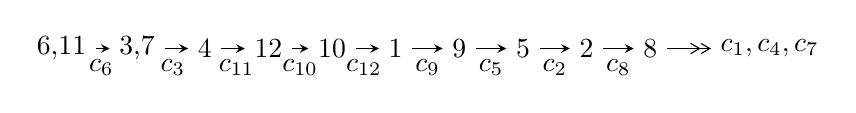
\begin{tikzpicture}[x=23pt, y=7pt]
	% node
	\node (A0) at (-1/8, 0) {6,11};
	\node (A1) at (17/16, 0) {3,7};
	\node (A2) at (17/8, 0) {4};
	\node (A3) at (25/8, 0) {12};
	\node (A4) at (33/8, 0) {10};
	\node (A5) at (41/8, 0) {1};
	\node (A6) at (49/8, 0) {9};
	\node (A7) at (57/8, 0) {5};
	\node (A8) at (65/8, 0) {2};
	\node (A9) at (73/8, 0) {8};
	\node (C1) at (1/2, -1) {$c_{6}$};
	\node (C2) at (13/8, -1) {$c_{3}$};
	\node (C3) at (21/8, -1) {$c_{11}$};
	\node (C4) at (29/8, -1) {$c_{10}$};
	\node (C5) at (37/8, -1) {$c_{12}$};
	\node (C6) at (45/8, -1) {$c_{9}$};
	\node (C7) at (53/8, -1) {$c_{5}$};
	\node (C8) at (61/8, -1) {$c_{2}$};
	\node (C9) at (69/8, -1) {$c_{8}$};
	\node (A10) at (11, 0) {$c_{1},c_{4},c_{7}$};

	% edge
	\draw[->,>=stealth]	
	(A0) edge (A1) (A1) edge (A2) (A2) edge (A3) (A3) edge (A4) (A4) edge (A5) (A5) edge (A6) (A6) edge (A7) (A7) edge (A8) (A8) edge (A9) ;
	\draw[->>,>={angle 60}]	
	(A9) edge (A10);
\end{tikzpicture} \\ 

\end{tabular} \\

\footnotetext{
The image of knot diagram is generated by the software ``\textbf{Draw programme}" developed by Andrew Bartholomew(\url{http://www.layer8.co.uk/maths/draw/index.htm\#Running-draw}), where we modified some parts for our purpose(\url{https://github.com/CATsTAILs/LinksPainter}).
}\phantom \\ \newline 
\centering \textbf{Ideals for irreducible components\footnotemark of $X_{\text{par}}$} 
 
\begin{align*}
I^u_{1}&=\langle 
- u^{51}- u^{50}+\cdots+b-1,\;-2 u^{51}-2 u^{50}+\cdots+a-3,\;u^{52}+2 u^{51}+\cdots+2 u+1\rangle \\
I^u_{2}&=\langle 
u^7- u^5+2 u^3+b- u+1,\;u^7- u^5+u^4+2 u^3- u^2+a+2,\;u^8- u^7- u^6+2 u^5+u^4-2 u^3+2 u-1\rangle \\
\\
\end{align*}
\raggedright * 2 irreducible components of $\dim_{\mathbb{C}}=0$, with total 60 representations.\\
\footnotetext{All coefficients of polynomials are rational numbers. But the coefficients are sometimes approximated in decimal forms when there is not enough margin.}
\newpage
\renewcommand{\arraystretch}{1}
\centering \section*{I. $I^u_{1}= \langle - u^{51}- u^{50}+\cdots+b-1,\;-2 u^{51}-2 u^{50}+\cdots+a-3,\;u^{52}+2 u^{51}+\cdots+2 u+1 \rangle$}
\flushleft \textbf{(i) Arc colorings}\\
\begin{tabular}{m{7pt} m{180pt} m{7pt} m{180pt} }
\flushright $a_{6}=$&$\begin{pmatrix}1\\0\end{pmatrix}$ \\
\flushright $a_{11}=$&$\begin{pmatrix}0\\u\end{pmatrix}$ \\
\flushright $a_{3}=$&$\begin{pmatrix}2 u^{51}+2 u^{50}+\cdots-3 u+3\\u^{51}+u^{50}+\cdots-2 u^2+1\end{pmatrix}$ \\
\flushright $a_{7}=$&$\begin{pmatrix}1\\u^2\end{pmatrix}$ \\
\flushright $a_{4}=$&$\begin{pmatrix}u^{51}-8 u^{49}+\cdots-5 u+2\\2 u^{51}+u^{50}+\cdots+u+1\end{pmatrix}$ \\
\flushright $a_{12}=$&$\begin{pmatrix}- u\\- u^3+u\end{pmatrix}$ \\
\flushright $a_{10}=$&$\begin{pmatrix}u^3\\u^5- u^3+u\end{pmatrix}$ \\
\flushright $a_{1}=$&$\begin{pmatrix}- u^5- u\\- u^7+u^5-2 u^3+u\end{pmatrix}$ \\
\flushright $a_{9}=$&$\begin{pmatrix}u^5+u\\u^5- u^3+u\end{pmatrix}$ \\
\flushright $a_{5}=$&$\begin{pmatrix}- u^{10}+u^8-2 u^6+u^4- u^2+1\\- u^{10}+2 u^8-3 u^6+2 u^4- u^2\end{pmatrix}$ \\
\flushright $a_{2}=$&$\begin{pmatrix}u^{51}+u^{50}+\cdots-4 u+3\\u^{51}+u^{50}+\cdots+u+1\end{pmatrix}$ \\
\flushright $a_{8}=$&$\begin{pmatrix}- u^{15}+2 u^{13}-4 u^{11}+4 u^9-4 u^7+4 u^5-2 u^3+2 u\\- u^{15}+3 u^{13}-6 u^{11}+7 u^9-6 u^7+4 u^5-2 u^3+u\end{pmatrix}$\\&\end{tabular}
\flushleft \textbf{(ii) Obstruction class $= -1$}\\~\\
\flushleft \textbf{(iii) Cusp Shapes $= - u^{51}+2 u^{50}+\cdots-14 u-3$}\\~\\
\newpage\renewcommand{\arraystretch}{1}
\flushleft \textbf{(iv) u-Polynomials at the component}\newline \\
\begin{tabular}{m{50pt}|m{274pt}}
Crossings & \hspace{64pt}u-Polynomials at each crossing \\
\hline $$\begin{aligned}c_{1}\end{aligned}$$&$\begin{aligned}
&u^{52}+15 u^{51}+\cdots+34 u+1
\end{aligned}$\\
\hline $$\begin{aligned}c_{2},c_{4}\end{aligned}$$&$\begin{aligned}
&u^{52}-9 u^{51}+\cdots-10 u+1
\end{aligned}$\\
\hline $$\begin{aligned}c_{3},c_{7}\end{aligned}$$&$\begin{aligned}
&u^{52}- u^{51}+\cdots+640 u+256
\end{aligned}$\\
\hline $$\begin{aligned}c_{5},c_{8},c_{9}\end{aligned}$$&$\begin{aligned}
&u^{52}+2 u^{51}+\cdots+336 u+49
\end{aligned}$\\
\hline $$\begin{aligned}c_{6},c_{11}\end{aligned}$$&$\begin{aligned}
&u^{52}-2 u^{51}+\cdots-2 u+1
\end{aligned}$\\
\hline $$\begin{aligned}c_{10},c_{12}\end{aligned}$$&$\begin{aligned}
&u^{52}+18 u^{51}+\cdots+14 u+1
\end{aligned}$\\
\hline
\end{tabular}\\~\\
\newpage\renewcommand{\arraystretch}{1}
\flushleft \textbf{(v) Riley Polynomials at the component}\newline \\
\begin{tabular}{m{50pt}|m{274pt}}
Crossings & \hspace{64pt}Riley Polynomials at each crossing \\
\hline $$\begin{aligned}c_{1}\end{aligned}$$&$\begin{aligned}
&y^{52}+53 y^{51}+\cdots-706 y+1
\end{aligned}$\\
\hline $$\begin{aligned}c_{2},c_{4}\end{aligned}$$&$\begin{aligned}
&y^{52}-15 y^{51}+\cdots-34 y+1
\end{aligned}$\\
\hline $$\begin{aligned}c_{3},c_{7}\end{aligned}$$&$\begin{aligned}
&y^{52}-51 y^{51}+\cdots-1622016 y+65536
\end{aligned}$\\
\hline $$\begin{aligned}c_{5},c_{8},c_{9}\end{aligned}$$&$\begin{aligned}
&y^{52}-26 y^{51}+\cdots-65170 y+2401
\end{aligned}$\\
\hline $$\begin{aligned}c_{6},c_{11}\end{aligned}$$&$\begin{aligned}
&y^{52}-18 y^{51}+\cdots-14 y+1
\end{aligned}$\\
\hline $$\begin{aligned}c_{10},c_{12}\end{aligned}$$&$\begin{aligned}
&y^{52}+34 y^{51}+\cdots-14 y+1
\end{aligned}$\\
\hline
\end{tabular}\\~\\
\newpage\flushleft \textbf{(vi) Complex Volumes and Cusp Shapes}
$$\begin{array}{c|c|c}  
\text{Solutions to }I^u_{1}& \I (\text{vol} + \sqrt{-1}CS) & \text{Cusp shape}\\
 \hline 
\begin{aligned}
u &= \phantom{-}0.661298 + 0.748302 I \\
a &= -0.320274 + 0.754666 I \\
b &= -0.79199 - 1.48215 I\end{aligned}
 & \phantom{-}0.80822 + 2.47111 I & -6.26058 - 3.26854 I \\ \hline\begin{aligned}
u &= \phantom{-}0.661298 - 0.748302 I \\
a &= -0.320274 - 0.754666 I \\
b &= -0.79199 + 1.48215 I\end{aligned}
 & \phantom{-}0.80822 - 2.47111 I & -6.26058 + 3.26854 I \\ \hline\begin{aligned}
u &= -0.636633 + 0.816820 I \\
a &= \phantom{-}0.268660 + 0.935747 I \\
b &= \phantom{-}2.46939 - 1.06759 I\end{aligned}
 & \phantom{-}6.10406 - 8.66203 I & -5.62163 + 4.32258 I \\ \hline\begin{aligned}
u &= -0.636633 - 0.816820 I \\
a &= \phantom{-}0.268660 - 0.935747 I \\
b &= \phantom{-}2.46939 + 1.06759 I\end{aligned}
 & \phantom{-}6.10406 + 8.66203 I & -5.62163 - 4.32258 I \\ \hline\begin{aligned}
u &= -1.036160 + 0.045183 I \\
a &= \phantom{-}0.56922 - 2.81424 I \\
b &= \phantom{-}0.23556 - 2.03154 I\end{aligned}
 & -4.76535 + 2.18839 I & -14.6770 - 3.6633 I \\ \hline\begin{aligned}
u &= -1.036160 - 0.045183 I \\
a &= \phantom{-}0.56922 + 2.81424 I \\
b &= \phantom{-}0.23556 + 2.03154 I\end{aligned}
 & -4.76535 - 2.18839 I & -14.6770 + 3.6633 I \\ \hline\begin{aligned}
u &= \phantom{-}0.723846 + 0.632329 I \\
a &= \phantom{-}0.194221 - 1.378370 I \\
b &= \phantom{-}1.63877 + 0.76596 I\end{aligned}
 & -0.43554 - 1.57909 I & -9.64188 + 1.77235 I \\ \hline\begin{aligned}
u &= \phantom{-}0.723846 - 0.632329 I \\
a &= \phantom{-}0.194221 + 1.378370 I \\
b &= \phantom{-}1.63877 - 0.76596 I\end{aligned}
 & -0.43554 + 1.57909 I & -9.64188 - 1.77235 I \\ \hline\begin{aligned}
u &= \phantom{-}1.04031\phantom{ +0.000000I} \\
a &= \phantom{-}0.375292\phantom{ +0.000000I} \\
b &= -0.518107\phantom{ +0.000000I}\end{aligned}
 & -6.36986\phantom{ +0.000000I} & -13.6620\phantom{ +0.000000I} \\ \hline\begin{aligned}
u &= -0.657608 + 0.692008 I \\
a &= \phantom{-}1.36055 - 0.47884 I \\
b &= \phantom{-}0.330991 - 0.978148 I\end{aligned}
 & -1.297150 - 0.510740 I & -6.51784 - 0.83295 I\\
 \hline 
 \end{array}$$\newpage$$\begin{array}{c|c|c}  
\text{Solutions to }I^u_{1}& \I (\text{vol} + \sqrt{-1}CS) & \text{Cusp shape}\\
 \hline 
\begin{aligned}
u &= -0.657608 - 0.692008 I \\
a &= \phantom{-}1.36055 + 0.47884 I \\
b &= \phantom{-}0.330991 + 0.978148 I\end{aligned}
 & -1.297150 + 0.510740 I & -6.51784 + 0.83295 I \\ \hline\begin{aligned}
u &= -0.666205 + 0.808385 I \\
a &= -0.331437 - 0.469968 I \\
b &= -2.08963 + 0.58134 I\end{aligned}
 & \phantom{-}7.27982 - 1.78274 I & -3.98925 - 0.13082 I \\ \hline\begin{aligned}
u &= -0.666205 - 0.808385 I \\
a &= -0.331437 + 0.469968 I \\
b &= -2.08963 - 0.58134 I\end{aligned}
 & \phantom{-}7.27982 + 1.78274 I & -3.98925 + 0.13082 I \\ \hline\begin{aligned}
u &= -0.806239 + 0.701530 I \\
a &= -0.587597 + 0.348457 I \\
b &= -0.210379 + 0.054742 I\end{aligned}
 & \phantom{-}2.80086 + 2.09505 I & -2.50659 - 3.48544 I \\ \hline\begin{aligned}
u &= -0.806239 - 0.701530 I \\
a &= -0.587597 - 0.348457 I \\
b &= -0.210379 - 0.054742 I\end{aligned}
 & \phantom{-}2.80086 - 2.09505 I & -2.50659 + 3.48544 I \\ \hline\begin{aligned}
u &= \phantom{-}1.063220 + 0.121546 I \\
a &= -2.29627 + 1.25450 I \\
b &= -1.38281 + 0.68102 I\end{aligned}
 & \phantom{-}0.93793 - 1.58244 I & -10.84568 + 1.37730 I \\ \hline\begin{aligned}
u &= \phantom{-}1.063220 - 0.121546 I \\
a &= -2.29627 - 1.25450 I \\
b &= -1.38281 - 0.68102 I\end{aligned}
 & \phantom{-}0.93793 + 1.58244 I & -10.84568 - 1.37730 I \\ \hline\begin{aligned}
u &= \phantom{-}0.549487 + 0.745372 I \\
a &= -0.521065 - 0.048868 I \\
b &= \phantom{-}0.799139 - 0.412000 I\end{aligned}
 & -1.81149 + 1.27627 I & -3.31406 - 1.04966 I \\ \hline\begin{aligned}
u &= \phantom{-}0.549487 - 0.745372 I \\
a &= -0.521065 + 0.048868 I \\
b &= \phantom{-}0.799139 + 0.412000 I\end{aligned}
 & -1.81149 - 1.27627 I & -3.31406 + 1.04966 I \\ \hline\begin{aligned}
u &= -0.973478 + 0.497457 I \\
a &= -1.35010 - 1.41893 I \\
b &= -0.920949 + 0.416007 I\end{aligned}
 & \phantom{-}3.12207 + 4.60453 I & -8.72425 - 5.65975 I\\
 \hline 
 \end{array}$$\newpage$$\begin{array}{c|c|c}  
\text{Solutions to }I^u_{1}& \I (\text{vol} + \sqrt{-1}CS) & \text{Cusp shape}\\
 \hline 
\begin{aligned}
u &= -0.973478 - 0.497457 I \\
a &= -1.35010 + 1.41893 I \\
b &= -0.920949 - 0.416007 I\end{aligned}
 & \phantom{-}3.12207 - 4.60453 I & -8.72425 + 5.65975 I \\ \hline\begin{aligned}
u &= \phantom{-}1.099660 + 0.097397 I \\
a &= \phantom{-}2.11231 - 2.23460 I \\
b &= \phantom{-}1.53001 - 1.70626 I\end{aligned}
 & -0.24824 - 8.05886 I & -12.40052 + 5.70179 I \\ \hline\begin{aligned}
u &= \phantom{-}1.099660 - 0.097397 I \\
a &= \phantom{-}2.11231 + 2.23460 I \\
b &= \phantom{-}1.53001 + 1.70626 I\end{aligned}
 & -0.24824 + 8.05886 I & -12.40052 - 5.70179 I \\ \hline\begin{aligned}
u &= -1.11145\phantom{ +0.000000I} \\
a &= \phantom{-}1.48524\phantom{ +0.000000I} \\
b &= \phantom{-}1.21896\phantom{ +0.000000I}\end{aligned}
 & -7.36266\phantom{ +0.000000I} & -8.96100\phantom{ +0.000000I} \\ \hline\begin{aligned}
u &= -0.905213 + 0.681246 I \\
a &= -0.523152 - 0.438777 I \\
b &= -0.1179880 - 0.0609129 I\end{aligned}
 & \phantom{-}2.49405 + 3.22105 I & -3.32606 - 3.39208 I \\ \hline\begin{aligned}
u &= -0.905213 - 0.681246 I \\
a &= -0.523152 + 0.438777 I \\
b &= -0.1179880 + 0.0609129 I\end{aligned}
 & \phantom{-}2.49405 - 3.22105 I & -3.32606 + 3.39208 I \\ \hline\begin{aligned}
u &= \phantom{-}0.856090 + 0.776847 I \\
a &= -0.786022 - 0.932466 I \\
b &= -0.57351 - 1.38717 I\end{aligned}
 & \phantom{-}10.43740 + 0.66966 I & -3.01264 + 0. I\phantom{ +0.000000I} \\ \hline\begin{aligned}
u &= \phantom{-}0.856090 - 0.776847 I \\
a &= -0.786022 + 0.932466 I \\
b &= -0.57351 + 1.38717 I\end{aligned}
 & \phantom{-}10.43740 - 0.66966 I & -3.01264 + 0. I\phantom{ +0.000000I} \\ \hline\begin{aligned}
u &= -1.015300 + 0.553492 I \\
a &= \phantom{-}1.73668 + 0.33530 I \\
b &= \phantom{-}0.221364 - 1.300870 I\end{aligned}
 & \phantom{-}2.49928 - 1.45715 I & -9.46738 + 0. I\phantom{ +0.000000I} \\ \hline\begin{aligned}
u &= -1.015300 - 0.553492 I \\
a &= \phantom{-}1.73668 - 0.33530 I \\
b &= \phantom{-}0.221364 + 1.300870 I\end{aligned}
 & \phantom{-}2.49928 + 1.45715 I & -9.46738 + 0. I\phantom{ +0.000000I}\\
 \hline 
 \end{array}$$\newpage$$\begin{array}{c|c|c}  
\text{Solutions to }I^u_{1}& \I (\text{vol} + \sqrt{-1}CS) & \text{Cusp shape}\\
 \hline 
\begin{aligned}
u &= \phantom{-}0.972910 + 0.643628 I \\
a &= -1.12101 - 2.08154 I \\
b &= \phantom{-}1.67842 - 1.59230 I\end{aligned}
 & -1.23183 - 3.44766 I & -10.73445 + 3.25709 I \\ \hline\begin{aligned}
u &= \phantom{-}0.972910 - 0.643628 I \\
a &= -1.12101 + 2.08154 I \\
b &= \phantom{-}1.67842 + 1.59230 I\end{aligned}
 & -1.23183 + 3.44766 I & -10.73445 - 3.25709 I \\ \hline\begin{aligned}
u &= \phantom{-}0.884417 + 0.769320 I \\
a &= \phantom{-}1.04291 + 1.44163 I \\
b &= -0.05794 + 1.42188 I\end{aligned}
 & \phantom{-}10.35090 - 6.48169 I & -3.29234 + 5.33033 I \\ \hline\begin{aligned}
u &= \phantom{-}0.884417 - 0.769320 I \\
a &= \phantom{-}1.04291 - 1.44163 I \\
b &= -0.05794 - 1.42188 I\end{aligned}
 & \phantom{-}10.35090 + 6.48169 I & -3.29234 - 5.33033 I \\ \hline\begin{aligned}
u &= -0.995994 + 0.663488 I \\
a &= -0.447793 + 0.743729 I \\
b &= -0.197171 + 1.217400 I\end{aligned}
 & -2.30244 + 5.77043 I & -8.73703 - 4.68081 I \\ \hline\begin{aligned}
u &= -0.995994 - 0.663488 I \\
a &= -0.447793 - 0.743729 I \\
b &= -0.197171 - 1.217400 I\end{aligned}
 & -2.30244 - 5.77043 I & -8.73703 + 4.68081 I \\ \hline\begin{aligned}
u &= \phantom{-}1.005230 + 0.684675 I \\
a &= \phantom{-}1.66351 + 1.36728 I \\
b &= -0.93378 + 1.89685 I\end{aligned}
 & -0.22005 - 7.93959 I & -8.35668 + 7.99048 I \\ \hline\begin{aligned}
u &= \phantom{-}1.005230 - 0.684675 I \\
a &= \phantom{-}1.66351 - 1.36728 I \\
b &= -0.93378 - 1.89685 I\end{aligned}
 & -0.22005 + 7.93959 I & -8.35668 - 7.99048 I \\ \hline\begin{aligned}
u &= \phantom{-}1.040490 + 0.652647 I \\
a &= \phantom{-}0.837700 - 0.810359 I \\
b &= \phantom{-}1.025560 + 0.617772 I\end{aligned}
 & -3.23709 - 6.60394 I & \phantom{-0.000000 } 0 \\ \hline\begin{aligned}
u &= \phantom{-}1.040490 - 0.652647 I \\
a &= \phantom{-}0.837700 + 0.810359 I \\
b &= \phantom{-}1.025560 - 0.617772 I\end{aligned}
 & -3.23709 + 6.60394 I & \phantom{-0.000000 } 0\\
 \hline 
 \end{array}$$\newpage$$\begin{array}{c|c|c}  
\text{Solutions to }I^u_{1}& \I (\text{vol} + \sqrt{-1}CS) & \text{Cusp shape}\\
 \hline 
\begin{aligned}
u &= -1.020440 + 0.711207 I \\
a &= -0.20228 - 2.51624 I \\
b &= -2.10957 - 0.88029 I\end{aligned}
 & \phantom{-}6.20768 + 7.49853 I & \phantom{-0.000000 } 0 \\ \hline\begin{aligned}
u &= -1.020440 - 0.711207 I \\
a &= -0.20228 + 2.51624 I \\
b &= -2.10957 + 0.88029 I\end{aligned}
 & \phantom{-}6.20768 - 7.49853 I & \phantom{-0.000000 } 0 \\ \hline\begin{aligned}
u &= -1.036210 + 0.704214 I \\
a &= -0.19781 + 3.00542 I \\
b &= \phantom{-}2.71533 + 1.45235 I\end{aligned}
 & \phantom{-}4.8974 + 14.3736 I & \phantom{-0.000000 } 0 \\ \hline\begin{aligned}
u &= -1.036210 - 0.704214 I \\
a &= -0.19781 - 3.00542 I \\
b &= \phantom{-}2.71533 - 1.45235 I\end{aligned}
 & \phantom{-}4.8974 - 14.3736 I & \phantom{-0.000000 } 0 \\ \hline\begin{aligned}
u &= -0.316269 + 0.673477 I \\
a &= \phantom{-}0.152937 - 1.157570 I \\
b &= \phantom{-}0.964431 + 0.772467 I\end{aligned}
 & \phantom{-}4.38303 + 5.94973 I & -5.70519 - 4.98093 I \\ \hline\begin{aligned}
u &= -0.316269 - 0.673477 I \\
a &= \phantom{-}0.152937 + 1.157570 I \\
b &= \phantom{-}0.964431 - 0.772467 I\end{aligned}
 & \phantom{-}4.38303 - 5.94973 I & -5.70519 + 4.98093 I \\ \hline\begin{aligned}
u &= \phantom{-}0.702232\phantom{ +0.000000I} \\
a &= -0.797304\phantom{ +0.000000I} \\
b &= \phantom{-}0.0429664\phantom{ +0.000000I}\end{aligned}
 & -1.05113\phantom{ +0.000000I} & -9.14920\phantom{ +0.000000I} \\ \hline\begin{aligned}
u &= -0.237887 + 0.635480 I \\
a &= -0.196476 + 0.636369 I \\
b &= -1.285860 - 0.135549 I\end{aligned}
 & \phantom{-}5.12115 - 0.59863 I & -4.16704 - 0.03207 I \\ \hline\begin{aligned}
u &= -0.237887 - 0.635480 I \\
a &= -0.196476 - 0.636369 I \\
b &= -1.285860 + 0.135549 I\end{aligned}
 & \phantom{-}5.12115 + 0.59863 I & -4.16704 + 0.03207 I \\ \hline\begin{aligned}
u &= \phantom{-}0.311034 + 0.368798 I \\
a &= -0.691540 - 1.071180 I \\
b &= \phantom{-}0.258704 + 0.649617 I\end{aligned}
 & -0.684234 - 1.109730 I & -7.41214 + 5.86160 I\\
 \hline 
 \end{array}$$\newpage$$\begin{array}{c|c|c}  
\text{Solutions to }I^u_{1}& \I (\text{vol} + \sqrt{-1}CS) & \text{Cusp shape}\\
 \hline 
\begin{aligned}
u &= \phantom{-}0.311034 - 0.368798 I \\
a &= -0.691540 + 1.071180 I \\
b &= \phantom{-}0.258704 - 0.649617 I\end{aligned}
 & -0.684234 + 1.109730 I & -7.41214 - 5.86160 I \\ \hline\begin{aligned}
u &= -0.359182\phantom{ +0.000000I} \\
a &= \phantom{-}3.20503\phantom{ +0.000000I} \\
b &= \phantom{-}0.863998\phantom{ +0.000000I}\end{aligned}
 & -2.10063\phantom{ +0.000000I} & \phantom{-}0.990710\phantom{ +0.000000I}\\
 \hline 
 \end{array}$$\newpage\newpage\renewcommand{\arraystretch}{1}
\centering \section*{II. $I^u_{2}= \langle u^7- u^5+2 u^3+b- u+1,\;u^7- u^5+u^4+2 u^3- u^2+a+2,\;u^8- u^7- u^6+2 u^5+u^4-2 u^3+2 u-1 \rangle$}
\flushleft \textbf{(i) Arc colorings}\\
\begin{tabular}{m{7pt} m{180pt} m{7pt} m{180pt} }
\flushright $a_{6}=$&$\begin{pmatrix}1\\0\end{pmatrix}$ \\
\flushright $a_{11}=$&$\begin{pmatrix}0\\u\end{pmatrix}$ \\
\flushright $a_{3}=$&$\begin{pmatrix}- u^7+u^5- u^4-2 u^3+u^2-2\\- u^7+u^5-2 u^3+u-1\end{pmatrix}$ \\
\flushright $a_{7}=$&$\begin{pmatrix}1\\u^2\end{pmatrix}$ \\
\flushright $a_{4}=$&$\begin{pmatrix}- u^7+u^5- u^4-2 u^3+u^2-2\\- u^7+u^5-2 u^3+u-1\end{pmatrix}$ \\
\flushright $a_{12}=$&$\begin{pmatrix}- u\\- u^3+u\end{pmatrix}$ \\
\flushright $a_{10}=$&$\begin{pmatrix}u^3\\u^5- u^3+u\end{pmatrix}$ \\
\flushright $a_{1}=$&$\begin{pmatrix}- u^5- u\\- u^7+u^5-2 u^3+u\end{pmatrix}$ \\
\flushright $a_{9}=$&$\begin{pmatrix}u^5+u\\u^5- u^3+u\end{pmatrix}$ \\
\flushright $a_{5}=$&$\begin{pmatrix}u^5+u\\u^7- u^5+2 u^3- u\end{pmatrix}$ \\
\flushright $a_{2}=$&$\begin{pmatrix}- u^7- u^4-2 u^3+u^2- u-2\\-2 u^7+2 u^5-4 u^3+2 u-1\end{pmatrix}$ \\
\flushright $a_{8}=$&$\begin{pmatrix}1\\u^2\end{pmatrix}$\\&\end{tabular}
\flushleft \textbf{(ii) Obstruction class $= 1$}\\~\\
\flushleft \textbf{(iii) Cusp Shapes $= -6 u^7+u^6+11 u^5-8 u^4-11 u^3+7 u^2+4 u-23$}\\~\\
\newpage\renewcommand{\arraystretch}{1}
\flushleft \textbf{(iv) u-Polynomials at the component}\newline \\
\begin{tabular}{m{50pt}|m{274pt}}
Crossings & \hspace{64pt}u-Polynomials at each crossing \\
\hline $$\begin{aligned}c_{1},c_{2}\end{aligned}$$&$\begin{aligned}
&(u-1)^8
\end{aligned}$\\
\hline $$\begin{aligned}c_{3},c_{7}\end{aligned}$$&$\begin{aligned}
&u^8
\end{aligned}$\\
\hline $$\begin{aligned}c_{4}\end{aligned}$$&$\begin{aligned}
&(u+1)^8
\end{aligned}$\\
\hline $$\begin{aligned}c_{5}\end{aligned}$$&$\begin{aligned}
&u^8+u^7-3 u^6-2 u^5+3 u^4+2 u-1
\end{aligned}$\\
\hline $$\begin{aligned}c_{6}\end{aligned}$$&$\begin{aligned}
&u^8- u^7- u^6+2 u^5+u^4-2 u^3+2 u-1
\end{aligned}$\\
\hline $$\begin{aligned}c_{8},c_{9}\end{aligned}$$&$\begin{aligned}
&u^8- u^7-3 u^6+2 u^5+3 u^4-2 u-1
\end{aligned}$\\
\hline $$\begin{aligned}c_{10}\end{aligned}$$&$\begin{aligned}
&u^8-3 u^7+7 u^6-10 u^5+11 u^4-10 u^3+6 u^2-4 u+1
\end{aligned}$\\
\hline $$\begin{aligned}c_{11}\end{aligned}$$&$\begin{aligned}
&u^8+u^7- u^6-2 u^5+u^4+2 u^3-2 u-1
\end{aligned}$\\
\hline $$\begin{aligned}c_{12}\end{aligned}$$&$\begin{aligned}
&u^8+3 u^7+7 u^6+10 u^5+11 u^4+10 u^3+6 u^2+4 u+1
\end{aligned}$\\
\hline
\end{tabular}\\~\\
\newpage\renewcommand{\arraystretch}{1}
\flushleft \textbf{(v) Riley Polynomials at the component}\newline \\
\begin{tabular}{m{50pt}|m{274pt}}
Crossings & \hspace{64pt}Riley Polynomials at each crossing \\
\hline $$\begin{aligned}c_{1},c_{2},c_{4}\end{aligned}$$&$\begin{aligned}
&(y-1)^8
\end{aligned}$\\
\hline $$\begin{aligned}c_{3},c_{7}\end{aligned}$$&$\begin{aligned}
&y^8
\end{aligned}$\\
\hline $$\begin{aligned}c_{5},c_{8},c_{9}\end{aligned}$$&$\begin{aligned}
&y^8-7 y^7+19 y^6-22 y^5+3 y^4+14 y^3-6 y^2-4 y+1
\end{aligned}$\\
\hline $$\begin{aligned}c_{6},c_{11}\end{aligned}$$&$\begin{aligned}
&y^8-3 y^7+7 y^6-10 y^5+11 y^4-10 y^3+6 y^2-4 y+1
\end{aligned}$\\
\hline $$\begin{aligned}c_{10},c_{12}\end{aligned}$$&$\begin{aligned}
&y^8+5 y^7+11 y^6+6 y^5-17 y^4-34 y^3-22 y^2-4 y+1
\end{aligned}$\\
\hline
\end{tabular}\\~\\
\newpage\flushleft \textbf{(vi) Complex Volumes and Cusp Shapes}
$$\begin{array}{c|c|c}  
\text{Solutions to }I^u_{2}& \I (\text{vol} + \sqrt{-1}CS) & \text{Cusp shape}\\
 \hline 
\begin{aligned}
u &= \phantom{-}0.570868 + 0.730671 I \\
a &= -0.805639 - 0.183365 I \\
b &= \phantom{-}0.320534 - 0.633953 I\end{aligned}
 & -2.68559 + 1.13123 I & -13.35119 - 0.17229 I \\ \hline\begin{aligned}
u &= \phantom{-}0.570868 - 0.730671 I \\
a &= -0.805639 + 0.183365 I \\
b &= \phantom{-}0.320534 + 0.633953 I\end{aligned}
 & -2.68559 - 1.13123 I & -13.35119 + 0.17229 I \\ \hline\begin{aligned}
u &= -0.855237 + 0.665892 I \\
a &= -0.189481 - 1.310380 I \\
b &= -1.54709 - 0.16160 I\end{aligned}
 & \phantom{-}0.51448 + 2.57849 I & -6.04880 - 3.90294 I \\ \hline\begin{aligned}
u &= -0.855237 - 0.665892 I \\
a &= -0.189481 + 1.310380 I \\
b &= -1.54709 + 0.16160 I\end{aligned}
 & \phantom{-}0.51448 - 2.57849 I & -6.04880 + 3.90294 I \\ \hline\begin{aligned}
u &= -1.09818\phantom{ +0.000000I} \\
a &= \phantom{-}0.729394\phantom{ +0.000000I} \\
b &= \phantom{-}0.879647\phantom{ +0.000000I}\end{aligned}
 & -8.14766\phantom{ +0.000000I} & -20.2760\phantom{ +0.000000I} \\ \hline\begin{aligned}
u &= \phantom{-}1.031810 + 0.655470 I \\
a &= \phantom{-}0.708845 - 0.169402 I \\
b &= \phantom{-}0.679246 + 0.851242 I\end{aligned}
 & -4.02461 - 6.44354 I & -15.5815 + 4.6831 I \\ \hline\begin{aligned}
u &= \phantom{-}1.031810 - 0.655470 I \\
a &= \phantom{-}0.708845 + 0.169402 I \\
b &= \phantom{-}0.679246 - 0.851242 I\end{aligned}
 & -4.02461 + 6.44354 I & -15.5815 - 4.6831 I \\ \hline\begin{aligned}
u &= \phantom{-}0.603304\phantom{ +0.000000I} \\
a &= -2.15684\phantom{ +0.000000I} \\
b &= -0.785038\phantom{ +0.000000I}\end{aligned}
 & -2.48997\phantom{ +0.000000I} & -20.7610\phantom{ +0.000000I}\\
 \hline 
 \end{array}$$\newpage
\newpage\renewcommand{\arraystretch}{1}
\centering \section*{ III. u-Polynomials}
\begin{tabular}{m{50pt}|m{274pt}}
Crossings & \hspace{64pt}u-Polynomials at each crossing \\
\hline $$\begin{aligned}c_{1}\end{aligned}$$&$\begin{aligned}
&((u-1)^8)(u^{52}+15 u^{51}+\cdots+34 u+1)
\end{aligned}$\\
\hline $$\begin{aligned}c_{2}\end{aligned}$$&$\begin{aligned}
&((u-1)^8)(u^{52}-9 u^{51}+\cdots-10 u+1)
\end{aligned}$\\
\hline $$\begin{aligned}c_{3},c_{7}\end{aligned}$$&$\begin{aligned}
&u^8(u^{52}- u^{51}+\cdots+640 u+256)
\end{aligned}$\\
\hline $$\begin{aligned}c_{4}\end{aligned}$$&$\begin{aligned}
&((u+1)^8)(u^{52}-9 u^{51}+\cdots-10 u+1)
\end{aligned}$\\
\hline $$\begin{aligned}c_{5}\end{aligned}$$&$\begin{aligned}
&(u^8+u^7-3 u^6-2 u^5+3 u^4+2 u-1)(u^{52}+2 u^{51}+\cdots+336 u+49)
\end{aligned}$\\
\hline $$\begin{aligned}c_{6}\end{aligned}$$&$\begin{aligned}
&(u^8- u^7+\cdots+2 u-1)(u^{52}-2 u^{51}+\cdots-2 u+1)
\end{aligned}$\\
\hline $$\begin{aligned}c_{8},c_{9}\end{aligned}$$&$\begin{aligned}
&(u^8- u^7-3 u^6+2 u^5+3 u^4-2 u-1)(u^{52}+2 u^{51}+\cdots+336 u+49)
\end{aligned}$\\
\hline $$\begin{aligned}c_{10}\end{aligned}$$&$\begin{aligned}
&(u^8-3 u^7+7 u^6-10 u^5+11 u^4-10 u^3+6 u^2-4 u+1)\\
&\cdot(u^{52}+18 u^{51}+\cdots+14 u+1)
\end{aligned}$\\
\hline $$\begin{aligned}c_{11}\end{aligned}$$&$\begin{aligned}
&(u^8+u^7+\cdots-2 u-1)(u^{52}-2 u^{51}+\cdots-2 u+1)
\end{aligned}$\\
\hline $$\begin{aligned}c_{12}\end{aligned}$$&$\begin{aligned}
&(u^8+3 u^7+7 u^6+10 u^5+11 u^4+10 u^3+6 u^2+4 u+1)\\
&\cdot(u^{52}+18 u^{51}+\cdots+14 u+1)
\end{aligned}$\\
\hline
\end{tabular}\newpage\renewcommand{\arraystretch}{1}
\centering \section*{ IV. Riley Polynomials}
\begin{tabular}{m{50pt}|m{274pt}}
Crossings & \hspace{64pt}Riley Polynomials at each crossing \\
\hline $$\begin{aligned}c_{1}\end{aligned}$$&$\begin{aligned}
&((y-1)^8)(y^{52}+53 y^{51}+\cdots-706 y+1)
\end{aligned}$\\
\hline $$\begin{aligned}c_{2},c_{4}\end{aligned}$$&$\begin{aligned}
&((y-1)^8)(y^{52}-15 y^{51}+\cdots-34 y+1)
\end{aligned}$\\
\hline $$\begin{aligned}c_{3},c_{7}\end{aligned}$$&$\begin{aligned}
&y^8(y^{52}-51 y^{51}+\cdots-1622016 y+65536)
\end{aligned}$\\
\hline $$\begin{aligned}c_{5},c_{8},c_{9}\end{aligned}$$&$\begin{aligned}
&(y^8-7 y^7+19 y^6-22 y^5+3 y^4+14 y^3-6 y^2-4 y+1)\\
&\cdot(y^{52}-26 y^{51}+\cdots-65170 y+2401)
\end{aligned}$\\
\hline $$\begin{aligned}c_{6},c_{11}\end{aligned}$$&$\begin{aligned}
&(y^8-3 y^7+7 y^6-10 y^5+11 y^4-10 y^3+6 y^2-4 y+1)\\
&\cdot(y^{52}-18 y^{51}+\cdots-14 y+1)
\end{aligned}$\\
\hline $$\begin{aligned}c_{10},c_{12}\end{aligned}$$&$\begin{aligned}
&(y^8+5 y^7+11 y^6+6 y^5-17 y^4-34 y^3-22 y^2-4 y+1)\\
&\cdot(y^{52}+34 y^{51}+\cdots-14 y+1)
\end{aligned}$\\
\hline
\end{tabular}
\vskip 2pc
\end{document}